\section{Bridge}

O padrão \textit{Bridge} permite variar as abstrações e as 
implementações de uma solução de forma independente, 
definindo uma interface que serve como ponte entre ambas. 
As operações da implementação são delegadas para essa 
nova interface, permitindo que as abstrações sejam 
implementadas sem precisar conhecer o tipo de 
implementação que está sendo utilizado. A estrutura do 
padrão pode ser vista na Figura \ref{bridge_struct}.\cite{gamma:1995}

\begin{figure}[htb]
	\caption{\label{bridge_struct}Estrutura do \textit{Bridge}.}
	\begin{center}
	    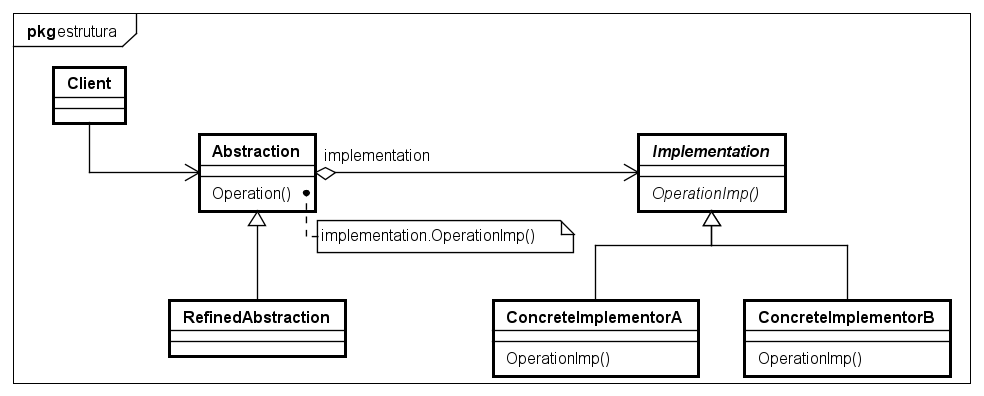
\includegraphics[scale=0.5]{5_padroes-contexto-funcional/5.2_estruturais/5.2.2_bridge/bridge_estrutura.png}
	\end{center}
  \caption*{Fonte: O Autor (2021)}
\end{figure}

\subsection*{Exemplo Orientado a Objetos}

Como exemplo, pode ser considerada a implementação de 
uma janela em um \textit{toolkit} para construir interfaces 
de usuários que permite o uso de implementações diferentes 
de janela: \textit{PM} e \textit{XWindow}. Além disso, é preciso definir tipos 
diferentes de janela, como janelas para ícones e janelas 
transitórias. Para que não seja necessário implementar 
uma versão diferente de janela de ícone e transitória 
para cada implementação diferente de janela, o padrão 
\textit{Bridge} pode ser usado para separar a implementação 
da abstração em duas hierarquias diferentes. O diagrama 
de classes da Figura \ref{bridge_exemplo} e o Código 
\ref{oobridge} demonstram o uso do padrão para esse 
exemplo.

\begin{figure}[htb]
	\caption{\label{bridge_exemplo}Exemplo de \textit{Bridge}.}
	\begin{center}
	    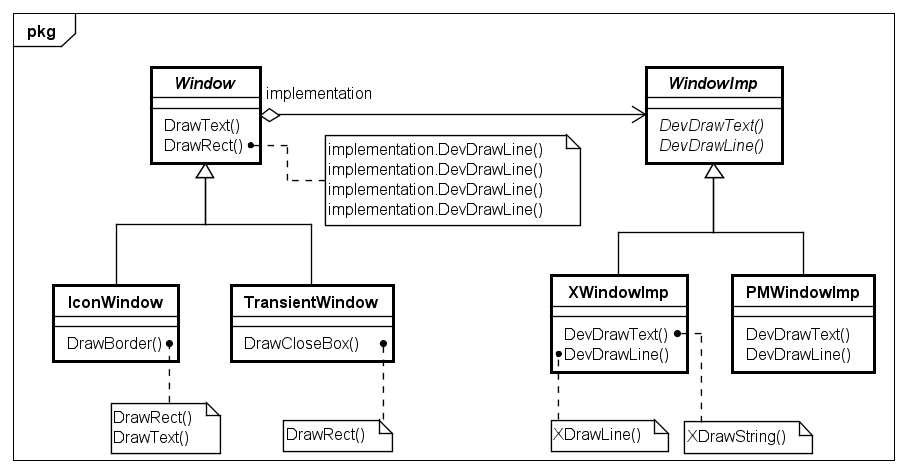
\includegraphics[scale=0.5]{5_padroes-contexto-funcional/5.2_estruturais/5.2.2_bridge/bridge_exemplo.png}
	\end{center}
  \caption*{Fonte: O Autor (2021)}
\end{figure}

\begin{lstlisting}[caption={\textit{Bridge} Orientado a Objetos.},label=oobridge]

abstract class Window(imp : WindowImp) {
  def DrawText() : Unit = {
    imp.DevDrawText()
  }

  def DrawRect() : Unit = {
    imp.DevDrawLine()
    imp.DevDrawLine()
    imp.DevDrawLine()
    imp.DevDrawLine()
  }
}

class IconWindow(imp : WindowImp) extends Window(imp) {
  def DrawBorder() : Unit = {
    DrawRect()
    DrawText()
  }
}

class TransientWindow(imp : WindowImp) extends Window(imp){
  def DrawCloseBox() : Unit = {
    DrawRect()
  }
}

trait WindowImp {
  def DevDrawText()
  def DevDrawLine()
}

class XWindowImp extends WindowImp {
  def DevDrawText() : Unit = {
    //Desenha texto para janela X
  }
  def DevDrawLine() : Unit = {
    //Desenha linha para janela X
  }
}

class PMWindowImp extends WindowImp {
  def DevDrawLine(): Unit = {
    //Desenha linha para janela PM
  }
  def DevDrawText(): Unit = {
    //Desenha texo para janela PM
  }
}

\end{lstlisting}
\legend{Fonte: O Autor (2021)}

\subsection*{Contexto Funcional}

Funções de alta ordem também podem ser utilizadas 
para separar as abstrações das implementações. 
No Código \ref{fpbridgeabs}, são definidas nas 
linhas 2 e 10, respectivamente, as 
duas funções equivalentes aos métodos das 
classes \texttt{IconWindow} e \texttt{TransientWindow} do exemplo 
orientado a objetos. Ao invés de reutilizar 
funções de uma superclasse, as funções 
\texttt{DrawText} e \texttt{DrawRect} são recebidas por parâmetro.

\begin{lstlisting}[caption={Abstrações no \textit{Bridge} Funcional.},label=fpbridgeabs]
    
def DrawIconBorder(text : String,
                   height : Int, width : Int,
                   DrawText : String => Unit,
                   DrawRect : (Int, Int) => Unit) : Unit = {
  DrawText(text)
  DrawRect(height, width)
}

def DrawTransientCloseBox(height : Int, width : Int,
                          DrawRect : (Int, Int) => Unit) : Unit = {
  DrawRect(height, width)
}
    
\end{lstlisting}
\legend{Fonte: O Autor (2021)}

No Código \ref{fpbridgeimp}, são definidas as 
funções referentes às implementações diferentes 
de \texttt{Window}. Essas são as funções que podem ser 
passadas como parâmetro para as funções vistas 
no Código \ref{fpbridgeabs}. Dessa forma, as 
abstrações de \texttt{Window} tornam-se independentes 
da forma como ela é implementada, resolvendo 
o problema encontrado pelo padrão.

\begin{lstlisting}[caption={Implementações no \textit{Bridge} Funcional.},label=fpbridgeimp]
    
def XDrawLine(size : Int) : Unit = {
  // Desenha linha
}

def XDrawText(text : String) : Unit = {
  // Desenha texto
}

def PMDrawLine(size : Int) : Unit = {
  // Desenha linha
}

def PMDrawText(text : String) : Unit = {
  // Desenha texto
}
    
\end{lstlisting}
\legend{Fonte: O Autor (2021)}